%*****************************************
\chapter{A near-infrared spectroscopic database of high-redshift quasars}\label{ch:chapter02}
%*****************************************

Rest-frame optical quasar emission lines provide much information. 
This includes black hole masses and systemic redshifts. 
Rest-frame optical lines, including [\ion{O}{III}], \hb and \ha, are redshifted to infra-red wavelengths at redshifts $z\gtrsim$2. 
However, the number of quasars at these redshifts with near-infrared spectra is limited. 
This is unfortunate because the peak epoch of galaxy evolution is at redshifts $2\lesssim z \lesssim 4$. 

In this chapter I will describe the construction of a database containing 553 high redshift quasars. 
This is the largest sample constructed, and is invaluable in a number of investigation. 
Because of this I intend to publically release the data in the near future. 

\begin{figure}
    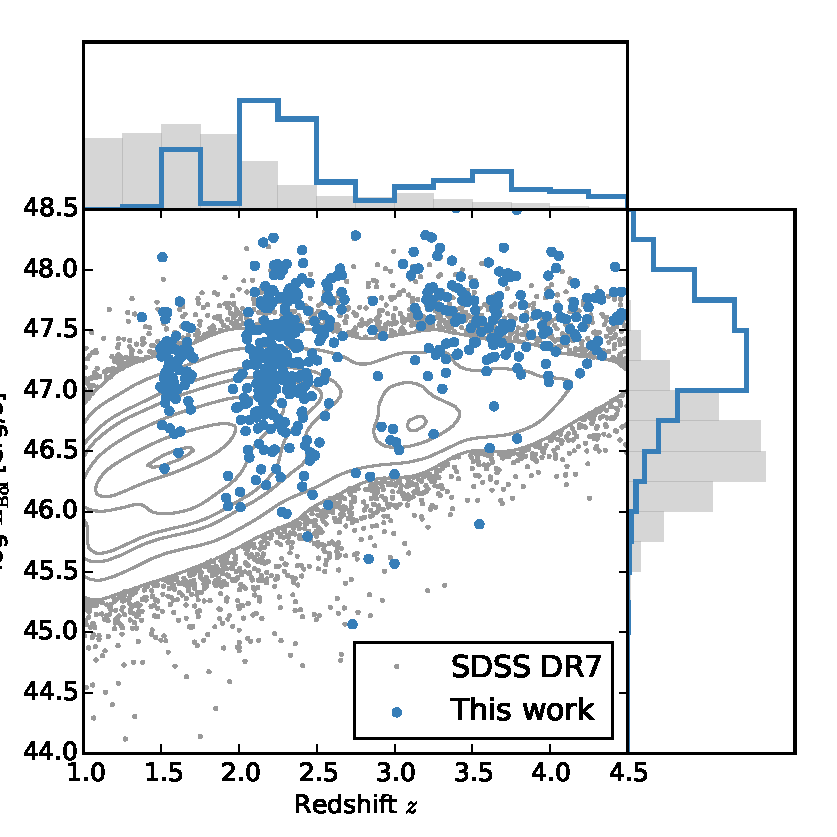
\includegraphics[width=0.8\columnwidth]{figures/chapter02/luminosity_z.pdf} 
    \caption{The ranges in redshift and luminosity covered by our sample, relative to the redshift-luminosity distribution of the SDSS DR7 quasar catalogue. In regions of high point-density, contours show equally-spaced lines of constant probability density generated using a Gaussian kernel-density estimator. For the SDSS sample we use \citet{hewett10} redshifts and bolometric luminosities measured by \citet{shen11}. For the quasars in this paper the redshift is defined using the peak of the \hans/\hb emission and the luminosity is measured in the continuum at 1350\AA\, and converted to a bolometric quantity using the same conversion factor employed by \citet{shen11}. Eight objects are missing because we do not have enough information to calculate the bolometric luminosity.}     
    \label{fig:lzplane}
\end{figure}

\begin{landscape}% Landscape page
    \centering % Center table
    \begin{minipage}{\linewidth}
    \renewcommand\footnoterule{}
    \captionof{table}{The numbers of quasars, the spectrographs and telescopes used to obtain the near-infrared spectra, and the instrumental configurations.}
    \begin{tabular}{ccccccc} 
    \hline
    Spectrograph & Telescope & Resolving power & Wavelength coverage & Slit width & Exposure times & Number \\
    & & $\lambda/\Delta\lambda$ & $\mu$m & arcsec & hr & \\  
    \hline
    FIRE       & MAGELLAN & 6000      & 0.80-2.50 & 0.6       & 0.5-1.0    & 18 \\
    GNIRS      & GEMINI-N & 5400      & 0.85-2.50 & 0.3-0.45 & 0.3-1.3  & 22 \\
    ISAAC      & VLT      & 5100      & 1.40-1.82 & 0.6       & 0.6-1.3  & 0  \\
    LIRIS      & WHT      & 945       & 1.39-2.42 & 1.0         & 0.2-0.8  & 15 \\
    NIRI       & GEMINI-N & 520-825   & 1.43-1.96 & 0.47-0.75 & 0.5-2.7 & 0 \\
    NIRSPEC    & Keck II  &           &           &           &         & 20 \\ 
    SINFONI    & VLT      & 2000-3000 & 1.10-2.45\footnote{$J$, $H$ or $K$ filters were employed to ensure     coverage of the \hbns/[\ion{O}{III}] spectral region.} &  & 0.1-0.7  & 2 \\
    SOFI       & NTT      & 1000-2000 & 1.53-2.52\footnote{Both the low resolution red grism and the medium     resolution grism, with $K$ and $H$ filters, were employed.} & 0.6       & 0.5-1.8  & 47 \\
    TRIPLESPEC & ARC-3.5m & 2500-3500 & 0.95-2.46 & 1.1-1.5   & 1.0-1.5    & 33 \\
    TRIPLESPEC & P200     & 2500-2700 & 1.00-2.40   & 1.0         &          & 23 \\
    XSHOOTER   & VLT      & 4350-7450 & 0.30-2.50   & 0.5-1.6   &     0.2-0.8     & 4 \\
    \hline
    \end{tabular}
    \end{minipage}
\end{landscape}




\section{Coatman et al. (2016) Quasars}

We selected quasars from the spectroscopic quasar catalogue of the Sloan Digital Sky Survey \citep[SDSS;][]{york00} Seventh Data Release \citep[DR7;][]{schneider10} with a wide range of \ion{C}{IV} blueshifts. 
The sample was restricted to objects with redshifts $2.14 < z <2.51$ (7,258 quasars), to ensure that the \hb and \ha emission lines fall within the $H$- and $K$-bands respectively, allowing us to observe both simultaneously with the appropriate grism configuration.
Given the limited number of quasars for which near-infrared spectra could be obtained, the quasar sample was further restricted to objects that are radio-quiet (5,980 quasars), show no evidence of broad absorption lines (BALs) in their spectra (5,299 quasars), and are free from significant dust extinction. 
We removed radio-loud objects from our sample using the same radio-loud classification as \citet{shen11}, and BAL quasars using the classifications of both \citet{shen11} and \citet{allen11}. 
The removal of quasars with significant dust extinction was achieved by identifying quasars with $i-K$ colours redder than a parametric spectral energy distributions (SED) model + SMC-like extinction curve with \ebv=0.05 \citep[see][]{maddox12}.
The $K$-magnitude was taken from the UKIRT Infrared Deep Sky Survey \citep[UKIDSS;][]{lawrence07} Large Area Survey (ULAS). 
The requirement to be in the ULAS footprint and have reliable $K$ band photometry reduced our sample of possible targets to 1,683, and the \ebv\, cut left 1,204 in our sample. 
Finally, a flux-limit of $K<18.5$ (AB) was applied to ensure that spectra of sufficient signal-to-noise ratio (S/N) could be obtained (412 quasars). 
 
We were able to obtain new infra-red spectra for 19 quasars from this sample of 412 possible targets (Section \ref{sec:observations}). 
The quasars included in this sub-sample were selected to have \ion{C}{IV}-emission shapes which span the full range observed in the population.
Reliably quantifying the distribution of \ion{C}{IV}-emission shapes has been made possible thanks to redshift-determination algorithms \citep[][Allen \& Hewett 2016, in preparation]{hewett10} which are independent of the \ion{C}{IV}-emission shape. 
Calculation of the \ion{C}{IV} emission line parameters is described in detail in the next section. 

Near-infrared spectra were obtained with the Long-slit Intermediate Resolution Infrared Spectrograph (LIRIS) mounted on the 4.2m William Herschel Telescope (WHT) at the Observatorio del Roque de los Muchachos (La Palma, Spain). 
Observations took place over four non-contiguous nights from 2015 March 31 to April 4. 
Approximately one night was lost due to poor weather and a further half-night was affected by poor transparency due to cloud. 
A one arcsecond slit-width was employed and the LIRIS $H+K$ low-resolution grism was selected, which covers the spectral ranges 1.53--1.79\,$\mu$m and 2.07--2.44\,$\mu$m with a dispersion of 9.7\AA/pixel. 
The spatial scale of the instrument is 0.25 arcsec/pixel. 
Observations were divided into 60\,s sub-exposures and performed in an ABBA nodding pattern, with the object placed at two positions along the slit 12 arcsec apart. 
Bright A0-5V stars were observed at similar air-masses to the targets in order to provide both telluric absorption corrections and a flux calibration of the quasar spectra.

The raw LIRIS data frames incorporate a known `pixel shift' which was first removed from all frames using the LIRIS data reduction package {\tt LIRISDR}. 
Subsequent data reduction was undertaken with standard {\tt IRAF}\footnote{IRAF is distributed by the National Optical Astronomy Observatory, which is operated by the Association of Universities for Research in Astronomy (AURA) under a cooperative agreement with the National Science Foundation.} procedures.  
The flat-field images, which were taken at the beginning of each night via illumination of the dome, were averaged and normalised to remove any wavelength-dependent signature. 
Each individual two-dimensional spectrum was then flat-field corrected. 
Consecutive AB and BA pairs of two-dimensional spectra were subtracted to remove the sky background. 
All the subtracted AB/BA-pairs for a target were then averaged to give the final two-dimensional spectrum.

The size of the one-dimensional spectrum extraction windows, in the slit direction, varied from 6-10 pixels. 
To increase the S/N, optimal variance-weighted extraction with sigma clipping was employed. 
For the fainter objects in our sample we were unable to trace the spectrum across the dispersion axis reliably and the trace from a telluric standard-star observation, observed at a similar air mass and time, was used instead. 
The wavelength calibration, using argon and xenon lamp exposures, resulted in root mean square errors in the range 1.01--1.71\,\AA, with a mean of 1.47\AA. 
The telluric standard star observations were reduced using the same steps described above. 
The stellar continuum was divided out of the standard star spectrum, which was then divided into the quasar spectrum to remove telluric absorption features. 
The spectral type and magnitude of the standard star were used to flux calibrate the quasar spectrum both in a relative and absolute sense.
Variable atmospheric conditions combined with the narrow slit width resulted in a significant level of uncertainty in the absolute flux calibration for the quasar observations. 
The use of the UKIDSS broadband magnitudes ($H$ and $K$) to normalise the spectra results in a significantly improved calibration. 

\section{Shen \& Liu (2012) and Shen (2016) Quasars}

\citet{shen16a} and \citet{shen12} obtained near-infrared spectroscopy for a sample of 74 luminous, $1.5 < z < 3.5$ quasars selected from the SDSS DR7 quasar catalogue. 
Targets had to possess good optical spectra covering the \ion{C}{IV} line and have redshifts $z\sim$ 1.5, 2.1, and 3.3 to ensure that the \hbns-[\ion{O}{iii}] region was covered in one of the near-infrared $JHK$ bands.
Thirty-eight of the quasars were observed with TripleSpec \citep{wilson04} on the Astrophysics Research Consortium (ARC) 3.5\,m telescope, and 36 with the Folded-port InfraRed Echellette \citep[FIRE;][]{simcoe10} on the 6.5\,m Magellan-Baade telescope.
The reduction of the spectra is described in \citet{shen16a} and \citet{shen12}. 

\section{Quasar Pairs}

Twenty per cent of our catalogue was observed as part of an ongoing effort to identify quasar pairs at very close projected separations \citep[Quasars Probing Quasars\footnote{www.ucolick.org/\textasciitilde xavier/QPQ/Quasars\_Probing\_Quasars} (QPQ);][]{hennawi06a,hennawi10}. 
The primary science driver of this work is to study the circum-galactic medium of the foreground quasars in absorption \citep{hennawi06b}.
Very accurate systemic redshift measurements are a requirement and a large amount of effort has gone into obtaining near-infrared spectra which cover low-ionisation broad lines or features from the quasar narrow line region \citep{prochaska09,lau15,hennawi15}. 
From the QPQ data set we identified 46 quasars with good-quality near-infrared spectra covering the \ha and/or \hb lines and SDSS and/or BOSS spectra covering the \ion{C}{IV} line. 
Twenty-two quasars were observed with the Gemini Near-Infrared Spectrograph \citep[GNIRS;][]{elias06} on the 8.1 m Gemini North telescope, 4 using the Infrared Spectrometer And Array Camera \citep[ISAAC;][]{moorwood98b} on the European Southern Observatory (ESO) Very Large Telescope (VLT), 11 with the Near InfraRed Imager and Spectrometer \citep[NIRI;][]{hodapp03} also on Gemini North and 9 with XSHOOTER \citep{vernet11}, again, on the VLT. 
The broad wavelength coverage of XSHOOTER means that the spectra cover the region from \ion{C}{IV} to \ha at the redshifts targeted. 
The XSHOOTER spectra have higher S/N and resolution than the SDSS/BOSS spectra in the rest-frame ultraviolet and therefore the XSHOOTER spectra are used by default to measure the \ion{C}{IV} emission. 

The  XSHOOTER  spectra  were  reduced  with  a  custom  software  package  developed  by  George  Becker \citep[for details, see][]{lau15}. 
The remaining data was processed with algorithms in the LowRedux\footnote{www.ucolick.org/\textasciitilde xavier/LowRedux} package \citep[see][]{prochaska09}.

\section{VLT SINFONI Quasars}

We performed a search of the ESO archive for high-$z$ quasars observed with the SINFONI  integral  field  spectrograph \citep{eisenhauer03,bonnet04} at VLT/UT4.
We found 79 quasars with redshifts $1.5 < z < 3.7$ which have $H$ and/or $K$ SINFONI spectroscopy, covering the \hb and \ha lines respectively. 
Seventy-two of the quasars are from a large programme led by L. Wisotzki (programme 083.B-0456(A)) to study the mass function and Eddington ratios of active BHs at redshifts $z\sim 2$ drawn from the Hamburg/ESO survey \citep{wisotzki00}.
A further seven SINFONI spectra are from a programme led by  J. D. Kurk (programme 090.B-0674(B)) to obtain reliable BH mass estimates from \hans/\hb for a sample of radio-loud/radio-quiet SDSS quasars.

The SINFONI spectra were reduced using the package EASYSINF\footnote{www.mrao.cam.ac.uk/\textasciitilde rw480/easysinf}.  
The package, which is based on the ESO-SINFONI pipeline, is described in \citet{williams16}. 

\section{ESO NTT SOFI Quasars}

Twelve per cent of the quasar catalogue derives from a large programme (programme 187.A-0645; PI: J. Hennawi) to combine near-infrared spectra from SOFI \citep{moorwood98a} on the 3.6\,m New Technology Telescope (NTT) with archival high-resolution optical spectra from the UV-Visual Echelle Spectrograph \citep[UVES;][]{dekker00} at VLT/UT2 and the High Resolution Echelle Spectrometer \citep[HIRES;][]{vogt94} at Keck to construct a legacy database of bright, high-redshift ($2 < z < 4$) quasars with both rest-frame optical spectra, covering the \hbns-[\ion{O}{III}] complex, and high-resolution rest-frame ultraviolet spectra.
The main science goal is to obtain precise systemic redshifts which are crucial for the study of absorption line systems.  
The SOFI spectra were reduced using a custom data reduction pipeline using algorithms in the LowRedux package.

Eighteen quasars have been targeted as part of the SDSS/BOSS spectroscopic quasar surveys.
In addition, 13 reduced and fluxed UVES spectra have been made available to us by A. Dall'Aglio (a description of the reduction procedure is contained in \citet{dallaglio08}).
The sample is larger ($\sim$100 quasars) but reduced UVES spectra providing rest-frame ultra-violet coverage of \ion{C}{IV} are not yet available for the remainder. 
The spectral resolution of the UVES observations is very high ($R$$\sim$40\,000) and the S/N of the spectra re-binned to a resolution of $\simeq$2000 is S/N$\simeq$300. 

Over five nights from 2015 August 31 to September 4 we obtained near-infrared SOFI spectra for a further 26 quasars (programme 095.B-0644(A); PI: L. Coatman). 
These quasars were selected from the SDSS DR7 quasar catalogue using criteria very similar to those described in Paper I (see Section~\ref{ss:paperI}). 
In particular, we selected quasars with large \ion{C}{IV} blueshifts to improve the statistics in this region of the \ion{C}{IV} emission-line parameter space. 

\section{Hale TripleSpec Quasars}

A further 36 quasars in our catalogue are bright SDSS quasars which were observed with the TRIPLESPEC spectrograph on the Palomar 200-inch Hale telescope (P200). 
The objects were observed with the same science goals as the SOFI NTT large programme. 
The spectra were reduced using a custom pipeline, again using algorithms in the LowRedux package. 


\begin{table*}
  \centering
  \vspace*{-0.4cm}
  \caption{The format of the table containing basic information on our sample. The full catalogue is available to download at the following URL.}
  \label{tab:nirdatabase}
  \vspace*{-0.1cm}
  \begin{minipage}{16cm}
  \centering
    \begin{tabular}{ccc} 
    \hline
    & Units & Description \\ 
    \hline
    NAME & & Name of spectra  \\
    DR7\_SPEC & & Name of SDSS/DR7 spectra \\
    DR12\_SPEC & & Name of BOSS/DR12 spectra \\
    ID & & Name of quasar (not unique) \\
    DATE & & Date near-infrared spectra acquired  \\
    RA & & \\
    DEC & & \\
    INSTR\_BAND & & Instrument configuration \\
    INSTR & & Instrument used \\
    z\_ICA & & \\
    z\_Line & & \\
    2massMag\_j & & \\
    2massMag\_h & & \\
    2massMag\_k & & \\
    2massMagErr\_j & & \\
    2massMagErr\_h & & \\
    2massMagErr\_k & & \\
    psfMag\_u & & \\
    psfMag\_g & & \\
    psfMag\_r & & \\
    psfMag\_i & & \\
    psfMag\_z & & \\
    psfMagErr\_u & & \\
    psfMagErr\_g & & \\
    psfMagErr\_r & & \\
    psfMagErr\_i & & \\
    psfMagErr\_z & & \\
    WISE\_W1MPRO & & \\
    WISE\_W2MPRO & & \\
    WISE\_W3MPRO & & \\
    WISE\_W4MPRO & & \\
    WISE\_W1SIGMPRO & & \\
    WISE\_W2SIGMPRO & & \\
    WISE\_W3SIGMPRO & & \\
    WISE\_W4SIGMPRO & & \\
    RADIO\_FLAG & & \\
    BAL\_FLAG & & \\
    \hline
    \end{tabular}
  \vspace*{-0.4cm}
  \end{minipage}
\end{table*}





